
\begin{figure*}[t!]
    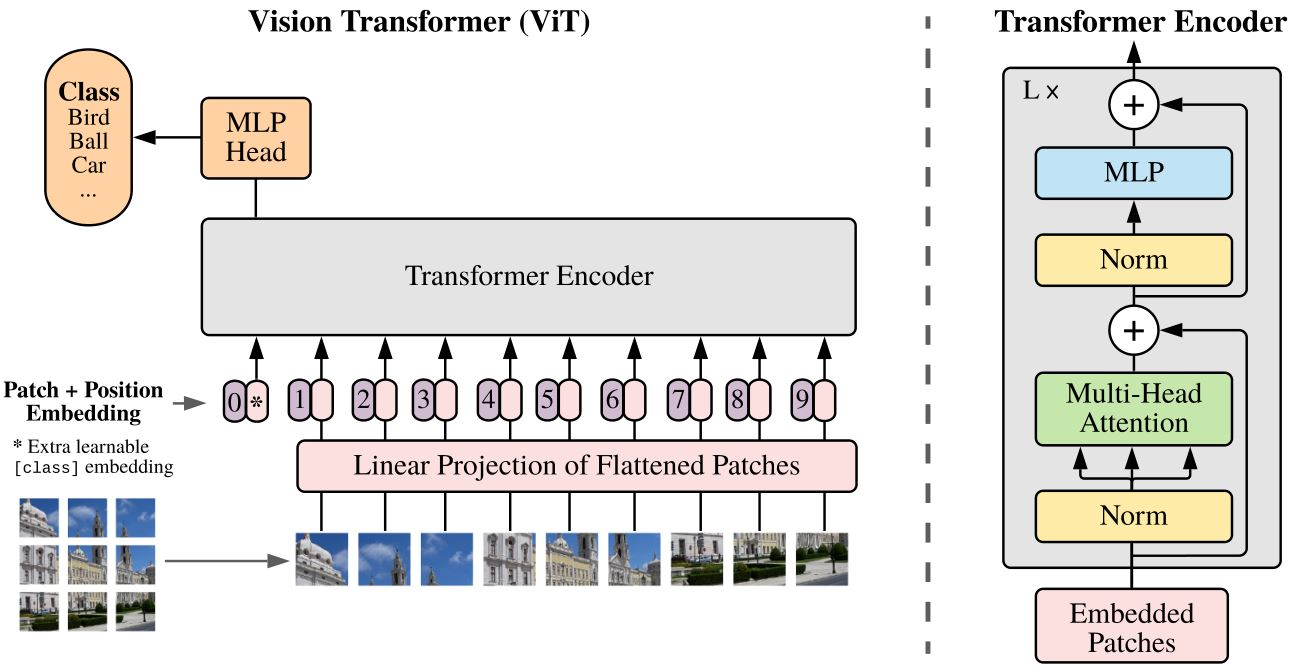
\includegraphics[width=\linewidth]{../images/ViT}
    \caption{ViT overview. An image is split into fixed-size patches, which are flattened and linearly projected into a sequence of vectors with positional embeddings. The sequence is then processed by a stack of transformer blocks, producing a sequence of vectors fed into a linear classifier. Illustration from \cite{dosovitskiy2021image}.}
    \label{fig:ViT}
    \centering
\end{figure*}

\section{Methods}
\label{sec:methods}

The use of UAVs in agriculture is not a new concept, but the introduction of VITs models has been a game changer in the field of Computer Vision (CV).
Unlike Multilayer Perceptrons (MLPs) and Convolutional Neural Networks (CNNs), ViTs excel at capturing intricate image patterns with their self-attention mechanism.
ViTs are highly scalable, reduce architectural complexity and support efficient transfer learning, therefore we decided to combine the two technologies to create a new solution for precision agriculture.

Our model design is based on the Vision Transformer architecture \cite{dosovitskiy2021image}.
In this section, we provide an overview of the architecture and the attention mechanism.

\subsection{Vision Transformer (ViT)}
\label{sec:ViT_overview}

The Vision Transformer is a variant of the transformer architecture, which was introduced by Vaswani et al. \cite{vaswani2023attention} for machine translation.

An overview of the model is depicted in fig.[\ref{fig:ViT}]. The standard Transformer receives as input a 1D sequence of token embeddings. To handle 2D images, the image $x \in \mathbb{R} ^{H\times W \times C}$ is reshaped into a sequence of flattened 2D patches $x_{p} \in \mathbb{R} ^{N\times(P^2\cdot C)}$, where $(H, W)$ is the resolution of the original image, $C$ is the number of channels, $(P, P)$ is the resolution of each image patch, and $N = HW/P^2$ is the resulting number of patches, which also serves as the effective input sequence length for the Transformer.

\begin{quote}
The Transformer uses constant latent vector size $D$ through all of its layers, so the patches are flattened and mapped to $D$ dimensions. The output of this projection is referred as the $patch$ $embeddings$.
Position embeddings are added to the patch embeddings to retain positional information. The resulting sequence of embedding vectors serves as input to the encoder\cite{dosovitskiy2021image}.
\end{quote}

The Transformer encoder \cite{vaswani2023attention} consists of alternating layers of Multiheaded Self-Attention (MSA) [\ref{subsec:MSA}] and MLP blocks. Layernorm (LN) \cite{ba2016layer} is applied before every block, and residual connections \cite{he2015deep} after every block.

\subsection{Multi-head self-attention (MSA)}
\label{subsec:MSA}

The attention mechanism is based on a trainable associative memory with (key, value) vector pairs.

A \textit{query} vector $q \in \mathbb{R} ^d$ is compared with each \textit{k key} vectors, packed into a matrix $K \in \mathbb{R} ^{k \times d}$, using inner products.
These inner products are then scaled and normalized with a softmax function to obtain $k$ weights.
The output of the attention is the weighted sum of a set of \textit{k value} vectors, packed into a matrix $V \in \mathbb{R} ^{k \times d}$.

For a sequence of \textit{N} query vectors packed into $Q \in \mathbb{R} ^{N \times d}$, it produces an output matrix (of size $N \times d$):
\begin{equation} \label{eq:attention} 
\text{Attention}(Q,K,V) = \text{Softmax}(QK^\intercal/\sqrt{d})V 
\end{equation}
where the Softmax function is applied to each row of the input matrix and the $\sqrt{d}$ term provides appropriate normalization. In \cite{vaswani2023attention} a Self-attention layer is proposed. Query, key and value matrices are themselves computed from a sequence of $N$ input vectors (packed into $X \in \mathbb{R} ^{N \times d}): Q = XW_{Q}, K = XW_{K}, V = XW_{V}$, by using linear transformations $W_{Q}, W_{K}, W_{V}$ with the constraint $k = N$, meaning that the attention is in between all the input vectors.
Finally, MSA layer is defined by considering $h$ attention $heads$, i.e., $h$ self-attention functions applied to the input. Each head provides a sequence of size $N \times d$.
These $h$ sequences are rearranged into a $N \times dh$ sequence that is reprojected by a linear layer into $N \times D$ \cite{touvron2021training}.

\subsection{Transfer Learning and Fine-tuning}
\label{subsec:TL-FT}

Our model implementation is based on the Lightning framework \cite{Falcon_PyTorch_Lightning_2019} which build upon \cite{paszke2019pytorch}.
It was pre-trained on a large image dataset\cite{deng2009imagenet} mostly used in classification tasks and fine-tuned by using the plots images extracted from the orthomosaic. Pretraining is useful because it allows us to leverage knowledge learned from a large dataset and apply it to a different task.
In our case, we used the pre-trained model to extract features from ImageNet and then fine-tuned it to our specific task.

To tailor the model for our regression task, we replaced the backbone's $head$ with a linear layer, which outputs a single-value output.

\subsection{Loss Function}
\label{subsec:loss_function}

We compared the performance of the model using different loss functions to measure the deviation of prediction from the actual value: the Huber Loss \cite{huber1964robust}, the Pseudo-Huber Loss \cite{girshick2015fast} and the Log Cosh Loss \cite{moshagen2021finding}.

All the loss functions act as a combination of linear and quadratic scorings, but they differ in the way they are combined.
The Huber Loss is a piecewise function that uses a hyperparameter delta $\delta$ to distinguish between linearity above and quadratic natures below it.

\begin{equation}
\label{eq:huber}
    \text{Huber}(y, \hat{y}) = \begin{cases}
    \frac{1}{2} \ast (y - \hat{y})^2 & \text{if } |y - \hat{y}| \leq \delta \\
    \delta \ast |y - \hat{y}| - \frac{1}{2} \ast \delta^2 & \text{otherwise}
    \end{cases}
\end{equation}

Similarly to the Huber Loss function \cite{huber1964robust}, the Log Cosh is a combination of linear and quadratic scorings as calculates the log of hyperbolic cosine of the error.

\begin{equation}
\label{eq:logcosh}
    \text{LogCosh}(y, \hat{y}) = \frac{1}{n} \sum_{n = 1}^{n} \log(\cosh(\hat{y} - y))
\end{equation}

Its implementation uses the $SoftPlus$ activation function, that is a smooth approximation to the ReLU function, and can be used to constrain the output of a machine to always be positive.

\begin{equation}
    \label{eq:softplus}
    \text{Softplus}(x) = \frac{1}{\beta} \ast \log(1 + \exp(\beta \ast x))
\end{equation}

Differently from the Huber Loss, Log Cosh is not a piecewise function, it is twice differentiable and it does not require the additional delta ($\delta$) hyperparameter to distinguish between linearity above and quadratic natures below it \ref{fig:LogCoshHuberLoss}.
Therefore, it has a considerable advantage over Huber loss for its property of continuity and differentiability.
It is, however, less adaptive than Huber loss due to the absence of any hyper-parameter.

\begin{figure}[t!]
    \includegraphics[width=\linewidth]{../images/LogCoshHuberLoss}
    \caption{LogCosh and HuberLoss functions.}
    \label{fig:LogCoshHuberLoss}
    \centering
\end{figure}

The Pseudo-Huber Loss is a smooth approximation to the Huber Loss function and is twice differentiable.
The main difference between the Log Cosh Loss and the Pseudo-Huber Loss functions is that the Log Cosh loss is always a quadratic function, while the pseudo-huber loss is a quadratic function for values of $|y - \hat{y}|$ below the threshold $\delta$ and a linear function for values of $|y - \hat{y}|$ above the threshold $\delta$.

\begin{equation}
L(y, \hat{y}) = \begin{cases}
    \frac{(y - \hat{y})^2}{2} & |y - \hat{y}| < \delta \\
    \delta |y - \hat{y}| - \frac{\delta^2}{2} & |y - \hat{y}| \ge \delta
    \end{cases}
\end{equation}

As mentioned, the Log Cosh loss has the advantage of being always a quadratic function, which makes it more efficient to optimize than the pseudo-huber loss. However, the Log Cosh loss may be less robust to outliers than the pseudo-huber loss.

The pseudo-huber loss has the advantage of being robust to outliers, which makes it a good choice for datasets that contain outliers. However, the pseudo-huber loss may be less efficient to optimize than the Log Cosh loss.

\subsection{Optimizer}
\label{subsec:optimizer}

The optimizer of choice is Adam \cite{kingma2017adam} that uses weight decay regularization.
Hutter pointed out in their paper \cite{loshchilov2019decoupled} that the weight decay is implemented wrongly in Adam and proposed a way to fix it.
\begin{equation}
\label{eq:first_moment}
m_t = \beta_1 m_{t-1} + (1 - \beta_1) g_t
\end{equation}
\begin{equation}
\label{eq:second_moment}
v_t = \beta_2 v_{t-1} + (1 - \beta_2) g_t^2
\end{equation}
\begin{equation}
\label{eq:weight_update}
w_t = w_{t-1} - \frac{lr}{1 - \beta_1^t} \cdot \frac{m_t}{\sqrt{v_t} + \epsilon}
\end{equation}
In the equations, $m_t$ and $v_t$ are the first and second moments of the gradient, $w_t$ is the weight at time step $t$, $g_t$ is the derivative of the cost with respect to $w_t$, $\beta_1$ and $\beta_2$ are the exponential decay rates for the moment estimates, $lr$ is the learning rate, $\epsilon$ is a small constant to prevent division by zero.